\section{AMIDST model class}

%---------------------------------------------------------------------
\subsection{Introduction and notation}
%---------------------------------------------------------------------

One of the main goals of AMIDST project is the definition of a general model class with the following characteristics: 

\begin{itemize}
\item It should be applicable to the three considered use-cases, i.e., Daimler, Cajamar, and Verdande,

\item it should be general enough to be applicable to any future, potentially similar, use-cases, and

\item it should be scalable supporting both inference and learning from massive data streams.
 
\end{itemize}

Taking these three different characteristics into account, we started the definition of the general model class by finding commonalities between all models presented and discussed in Section \ref{Section:PreliminaryModels}. Let's first introduce some new ``graphical notation''  to ease the model description process. This notation is based on the use of \textit{subnetwork modules}, i.e., some parts of the DBN with common features such as all the nodes are continuous and observed. Figure \ref{Figure:ModelClass:Notation} illustrates a visual description of this notation. As it can be seen, instead of circle or eclipsed nodes used to depict single variables in a graph, we represent here the subnetwork modules using square boxes. In addition, following a similar notation used previously for the different types of nodes in (see Figure \ref{Figure:PreliminariesNotation}), square boxes rounded by dashed lines refer to hidden subnetworks (i.e., including only hidden variables), while square boxes rounded by continuous lines refer to observed subnetworks (i.e., including only observed variables). Then, depending on the colour of the square boxes, subnetworks could be either discrete (green) or continuous (blue). 
% Square boxes can also be nested to represent smaller subcomponents inside a bigger subcomponent. 

\begin{figure}[ht!]
\begin{center}
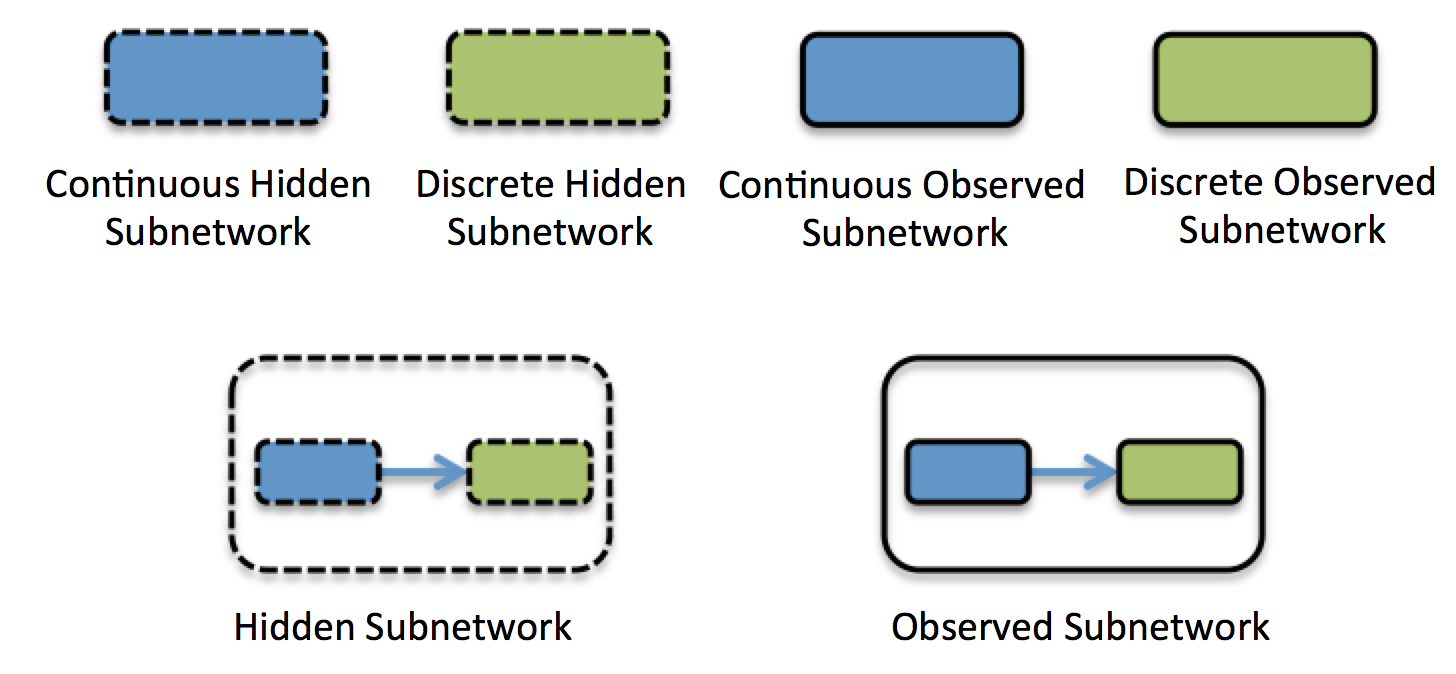
\includegraphics[scale=0.4]{./figures/ModelClass0}
\caption{\label{Figure:ModelClass:Notation} Graphical notation for the different potential subnetworks.}
\end{center}
\end{figure}

%---------------------------------------------------------------------
\subsection{The model classes of the three use-cases}
%---------------------------------------------------------------------

Using the new defined graphical notation, we re-introduce in this section the model classes of the three use-cases (that have been previously presented in Section \ref{Section:PreliminaryModels}). This model reinterpretation, using high-level descriptors, is crucial in order to identify the commonalities between all models. 

%---------------------------------------------------------------------
\subsubsection{Daimler model class}
%---------------------------------------------------------------------

Daimler's models have been previously described in Figures \ref{Figure:daimlerLEdynGeneric} and \ref{Figure:daimlerreldyn}. As commented in Section \ref{Section:DaimlerDynamic}, one the main issues of these current models is that they contain discrete children with continuous parents, and do not fall into the conditional linear Gaussian family \cite{JensenNielsen2007}. To deal with this problem, we adopt here the same solution pursed in \cite{kasper2012object} which consists in discretizing these nodes. In this way, the general structure of Daimler's models corresponds to the one depicted in Figure \ref{Figure:DaimlerModelClass}, where there is no more discrete children with continuous parents, and it is possible thereby to use standard parametrizations \cite{JensenNielsen2007}. 

\begin{figure}[ht!]
\begin{center}
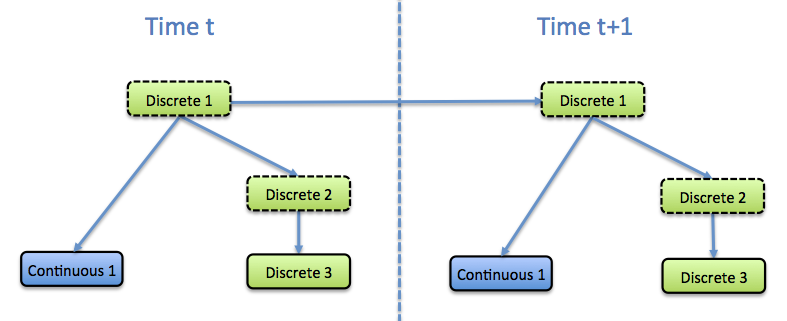
\includegraphics[scale=0.4]{./figures/DaimlerModelClass}
\caption{\label{Figure:DaimlerModelClass} Daimler model class}
\end{center}
\end{figure}

This general model is structured as a 2T-DBN (see Section \ref{SubSubSection:2DBNs}). The static model which is repeated over time consists of four elements: 

\begin{enumerate}
\item ``Discrete 1'': is a discrete hidden subnetwork which is the only element temporally connected
\item ``Discrete 2'': is an additional discrete hidden subnetwork which is not temporally connected. It is included only for modelling purposes inside a time slice
\item ``Discrete 3'': is an observed discrete subnetwork directly depending on ``Discrete 2'' subnetwork
\item  ``Continuous 1'': is an observed continuous subnetwork which is directly depending on ``Discrete 1'' subnetwork
\end{enumerate}

As commented, this 2T-DBN is only temporally connected through the hidden subnetwork on top. Consequently, the future and past time slices of our 2T-DBN are conditionally independent given the hidden subnetwork corresponding to the present time. Additionally, inside a time slice, the observed continuous and discrete subnetworks are also conditionally independent given this hidden subnetwork.

In addition, we have more structure that can be exploited during inference and which is not reflected in this meta-network. Specifically, the hidden and observed subnetworks may have a polytree structure \cite{JensenNielsen2007}. In this case, both static and dynamic BNs have polytree structure and this can be exploited during inference. 

%---------------------------------------------------------------------
\subsubsection{CajaMar model class}
%---------------------------------------------------------------------

Concerning CajaMar use-case, both application scenarios share the same models, of which two versions have been previously discussed, namely, static and dynamic (see Section \ref{Section:CajaMarModels}). 

At this point, we obviate the static version, because the general AMIDST model class is primarily a dynamic model class. Therefore, the high-level description of CajaMar's dynamic model is given in Figure \ref{Figure:CajaMarModelClass}. As it can be seen, CajaMar models is composed by four main subnetworks, which are expanded over time and all of them are observed. Hence, at CajaMar, there are no hidden subnetworks. 

\begin{figure}[ht!]
\begin{center}
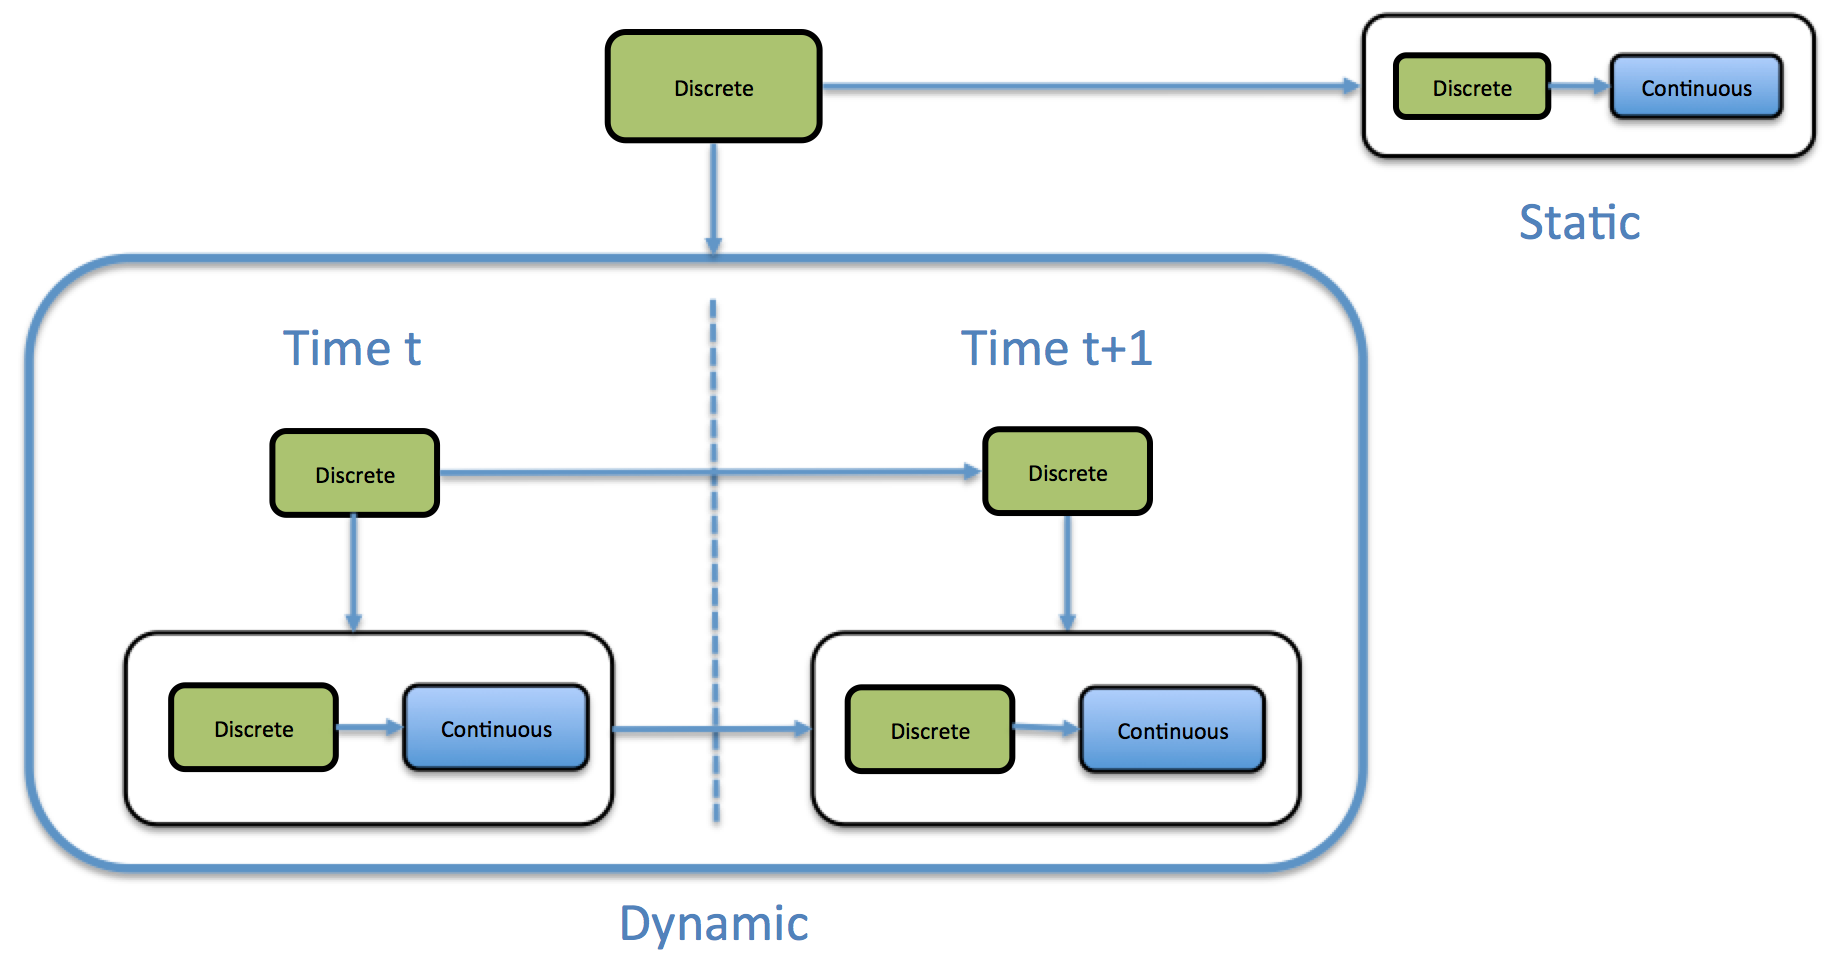
\includegraphics[scale=0.4]{./figures/CajaMarModelClass}
\caption{\label{Figure:CajaMarModelClass} CajaMar model class}
\end{center}
\end{figure}

%---------------------------------------------------------------------
\subsubsection{Verdande model class}
%---------------------------------------------------------------------

Verdande's models were visually described in Figures ?, ? and ? for the three identified application scenarios (see Section \ref{Section:VerdandeModels}). Figure \ref{Figure:VerdandeModelClass} visually depicts the high-level model class that subsumes the different models of the three application scenarios. As it can be seen, it is possible to distinguish three interpretations each corresponding to an application scenario:

\begin{itemize}
\item If we keep the subnetworks ``Discrete 2'', ``Continuous 1'' and ``Continuous 2'', we obtain the switching Kalman filter model for application scenario 1 (see Section \ref{SubSection:DetectionTorque}),
\item If we keep ``Continuous 1'', ``Discrete 3'' and ``Continuous 2'', we obtain the input-output Kalman filter model for application scenario 2 (see Section \ref{SubSection:SemiAutomaticLabelling}), and
\item finally, if we keep ``Discrete 1'', ``Discrete 2'' and ``Continuous 2'', we obtain the input-output Kalman filter model for application scenario 3  (see Section \ref{SubSection:DetectionFormation}).
\end{itemize}

\begin{figure}[ht!]
\begin{center}
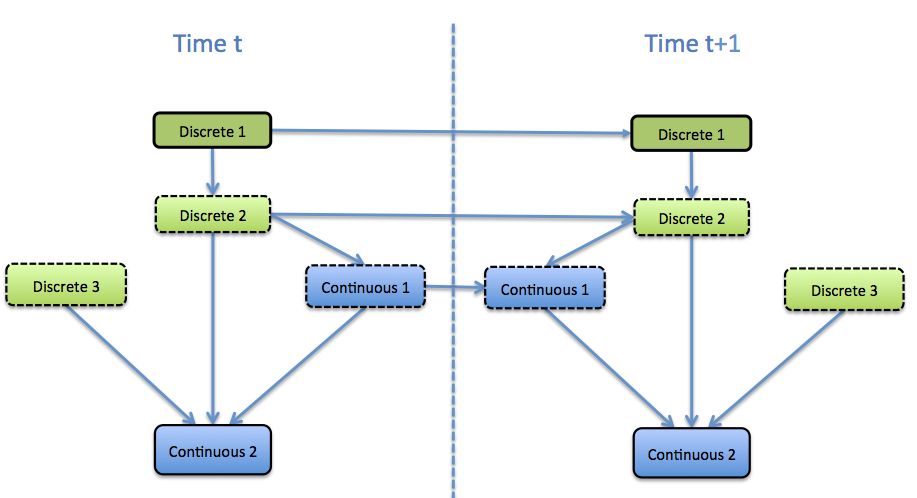
\includegraphics[scale=0.4]{./figures/VerdandeModelClass}
\caption{\label{Figure:VerdandeModelClass} Verdande model class}
\end{center}
\end{figure}

Similarly to the Daimler model, the general model is structured as a 2T-DBN (see Section \ref{SubSubSection:2DBNs}). The static part which is repeated over time is composed by five subnetworks: two observed components (i.e., one discrete temporally connected on the top, and one continuous at the bottom); and three hidden components in the middle (i.e., one hidden discrete and one hidden continuous both are temporally connected, and one hidden discrete, which is not temporally connected and its function is to account for the possible conditional dependencies of the observed continuous variables).  

However, contrary to Daimler, Verdande class model does not have a polytree structure that can be exploited during inference. 

%---------------------------------------------------------------------
\subsection{The general AMIDST model class}
%---------------------------------------------------------------------

\begin{figure}[ht!]
\begin{center}
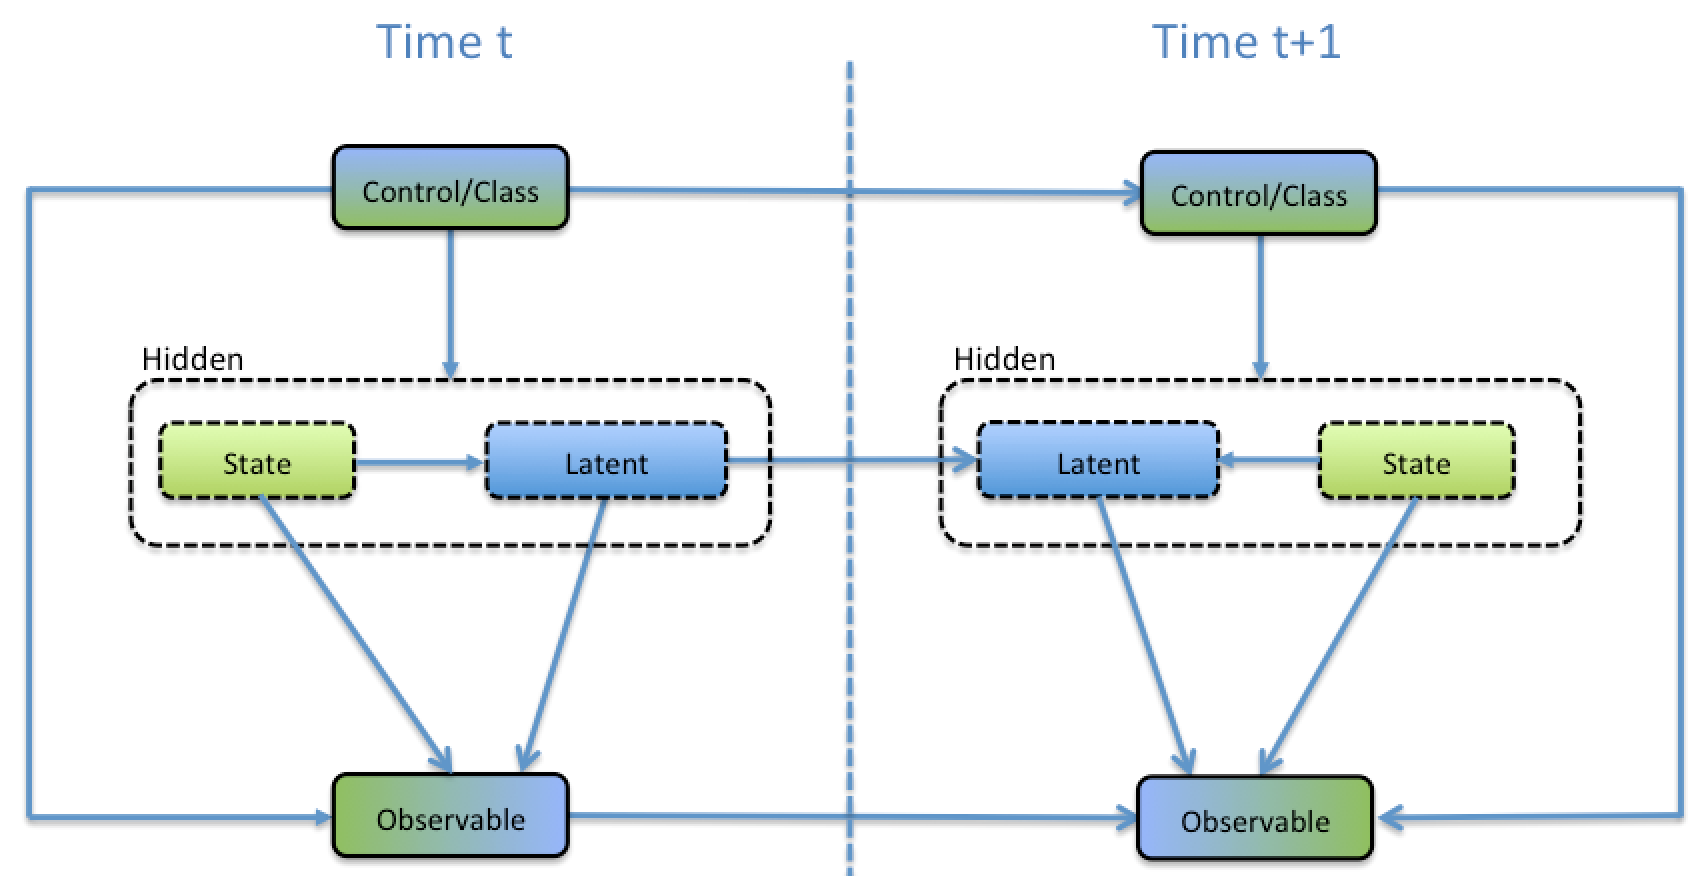
\includegraphics[scale=0.4]{./figures/AMIDSTModelClassGeneral}
\caption{\label{Figure:AMIDSTModelClassHighLevel} The general AMIDST model class}
\end{center}
\end{figure}

\begin{figure}[ht!]
\begin{center}
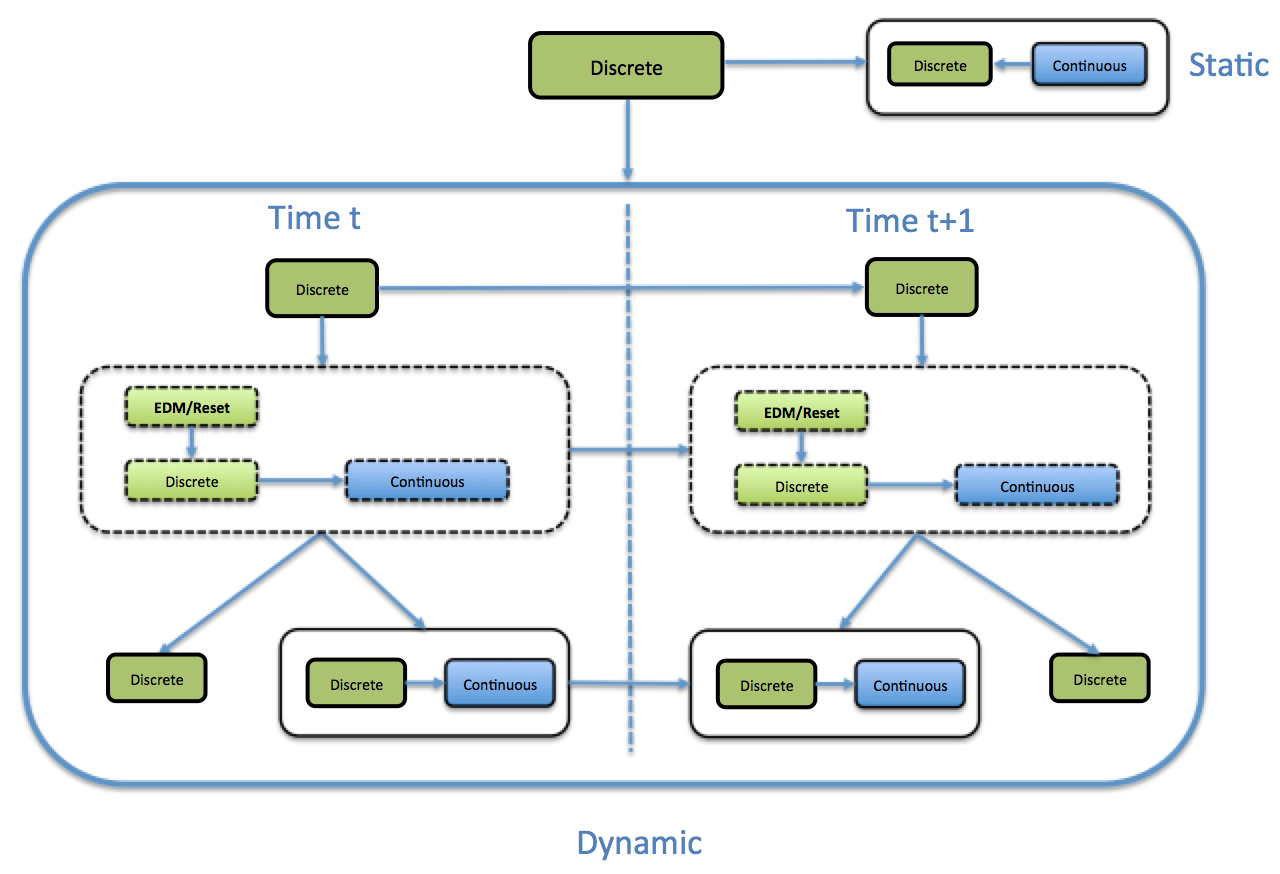
\includegraphics[scale=0.4]{./figures/AMIDSTModelClass}
\caption{\label{Figure:AMIDSTModelClass} AMIDST model class low level}
\end{center}
\end{figure}

\begin{figure}[ht!]
\begin{center}
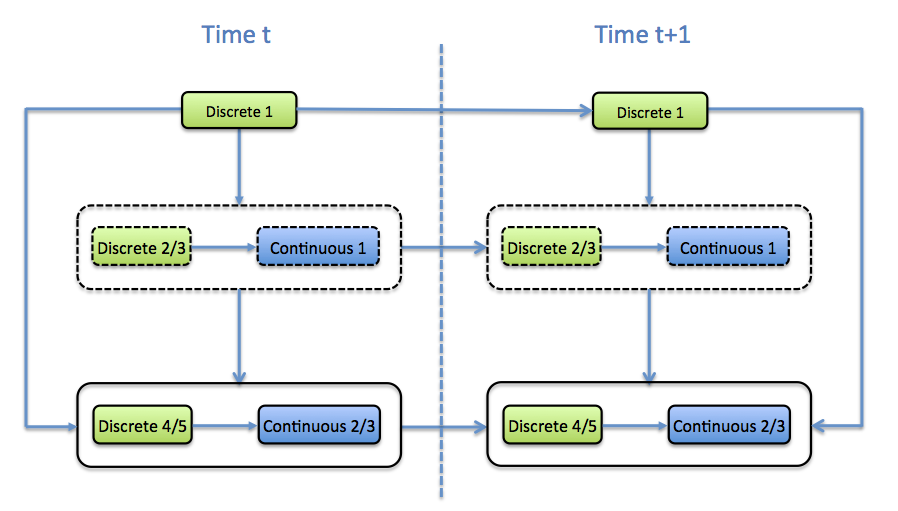
\includegraphics[scale=0.4]{./figures/AMIDSTModelClassHighLevel}
\caption{\label{Figure:AMIDSTModelClassHighLevel} AMIDST model class high level}
\end{center}
\end{figure}

\begin{figure}[ht!]
\begin{center}
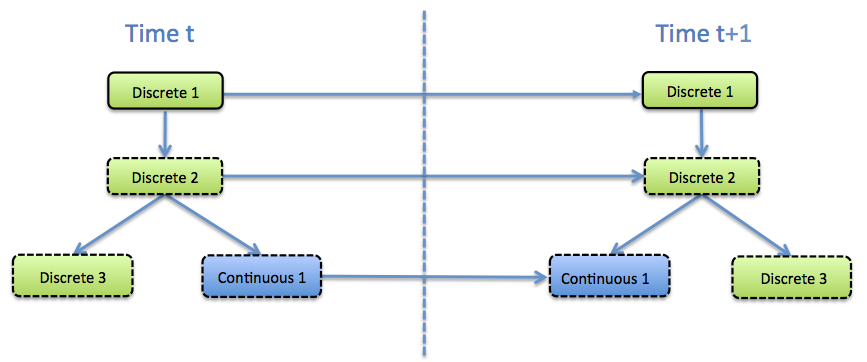
\includegraphics[scale=0.4]{./figures/AMIDSTModelClassTopPart}
\caption{\label{Figure:AMIDSTModelClassHighLevel} AMIDST model class top part}
\end{center}
\end{figure}

\begin{figure}[ht!]
\begin{center}
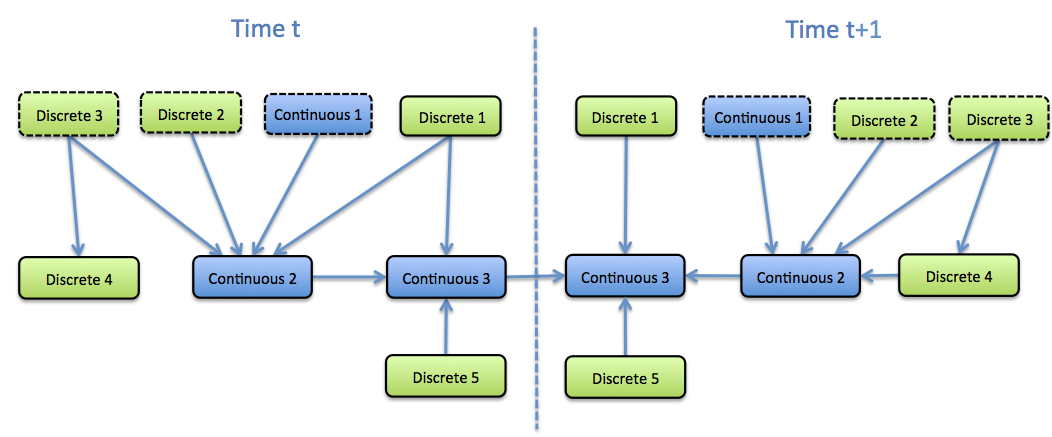
\includegraphics[scale=0.4]{./figures/AMIDSTModelClassLowPart}
\caption{\label{Figure:AMIDSTModelClassHighLevel} AMIDST model class low part}
\end{center}
\end{figure}